\documentclass[11pt,a4paper]{article}
\usepackage[margin=1in]{geometry}
\usepackage{fancyhdr}
\usepackage{graphicx}
\usepackage{amsmath,amssymb}
\usepackage{booktabs}
\usepackage{float}
\usepackage{caption}
\usepackage{hyperref}
\usepackage{enumitem}

\pagestyle{fancy}
\fancyhf{}
\fancyhead[L]{MAIE5102}
\fancyhead[R]{\footnotesize\textbf{THE HONG KONG}\\\footnotesize\textbf{UNIVERSITY OF SCIENCE}\\\footnotesize\textbf{AND TECHNOLOGY}}
\fancyfoot[C]{\thepage}
\renewcommand{\headrulewidth}{0pt}
\setlength{\headheight}{36pt}

\begin{document}

% Title page
\thispagestyle{empty}
\vspace*{8cm}
\begin{center}
{\Large MAIE5102:}\\[6pt]
{\large AI Fundamentals: Concepts and Methods}\\[24pt]
{\Large\textbf{Homework Assignment 1}}\\[18pt]
{\large Student ID: 21272577}\\[12pt]
\end{center}
\newpage

% ============================================================
\section{Question 1: Computation Graph (20 points)}

\textbf{Function:}
\[
f(x_0, x_1, x_2, x_3) = \frac{e^{x_3}}{(x_0 + 3x_1) \cdot x_2^2}
\]
\textbf{Given:} $x_0 = 1,\ x_1 = -1,\ x_2 = 2,\ x_3 = 16$

\subsection{Computation Graph}

\begin{figure}[H]
\centering
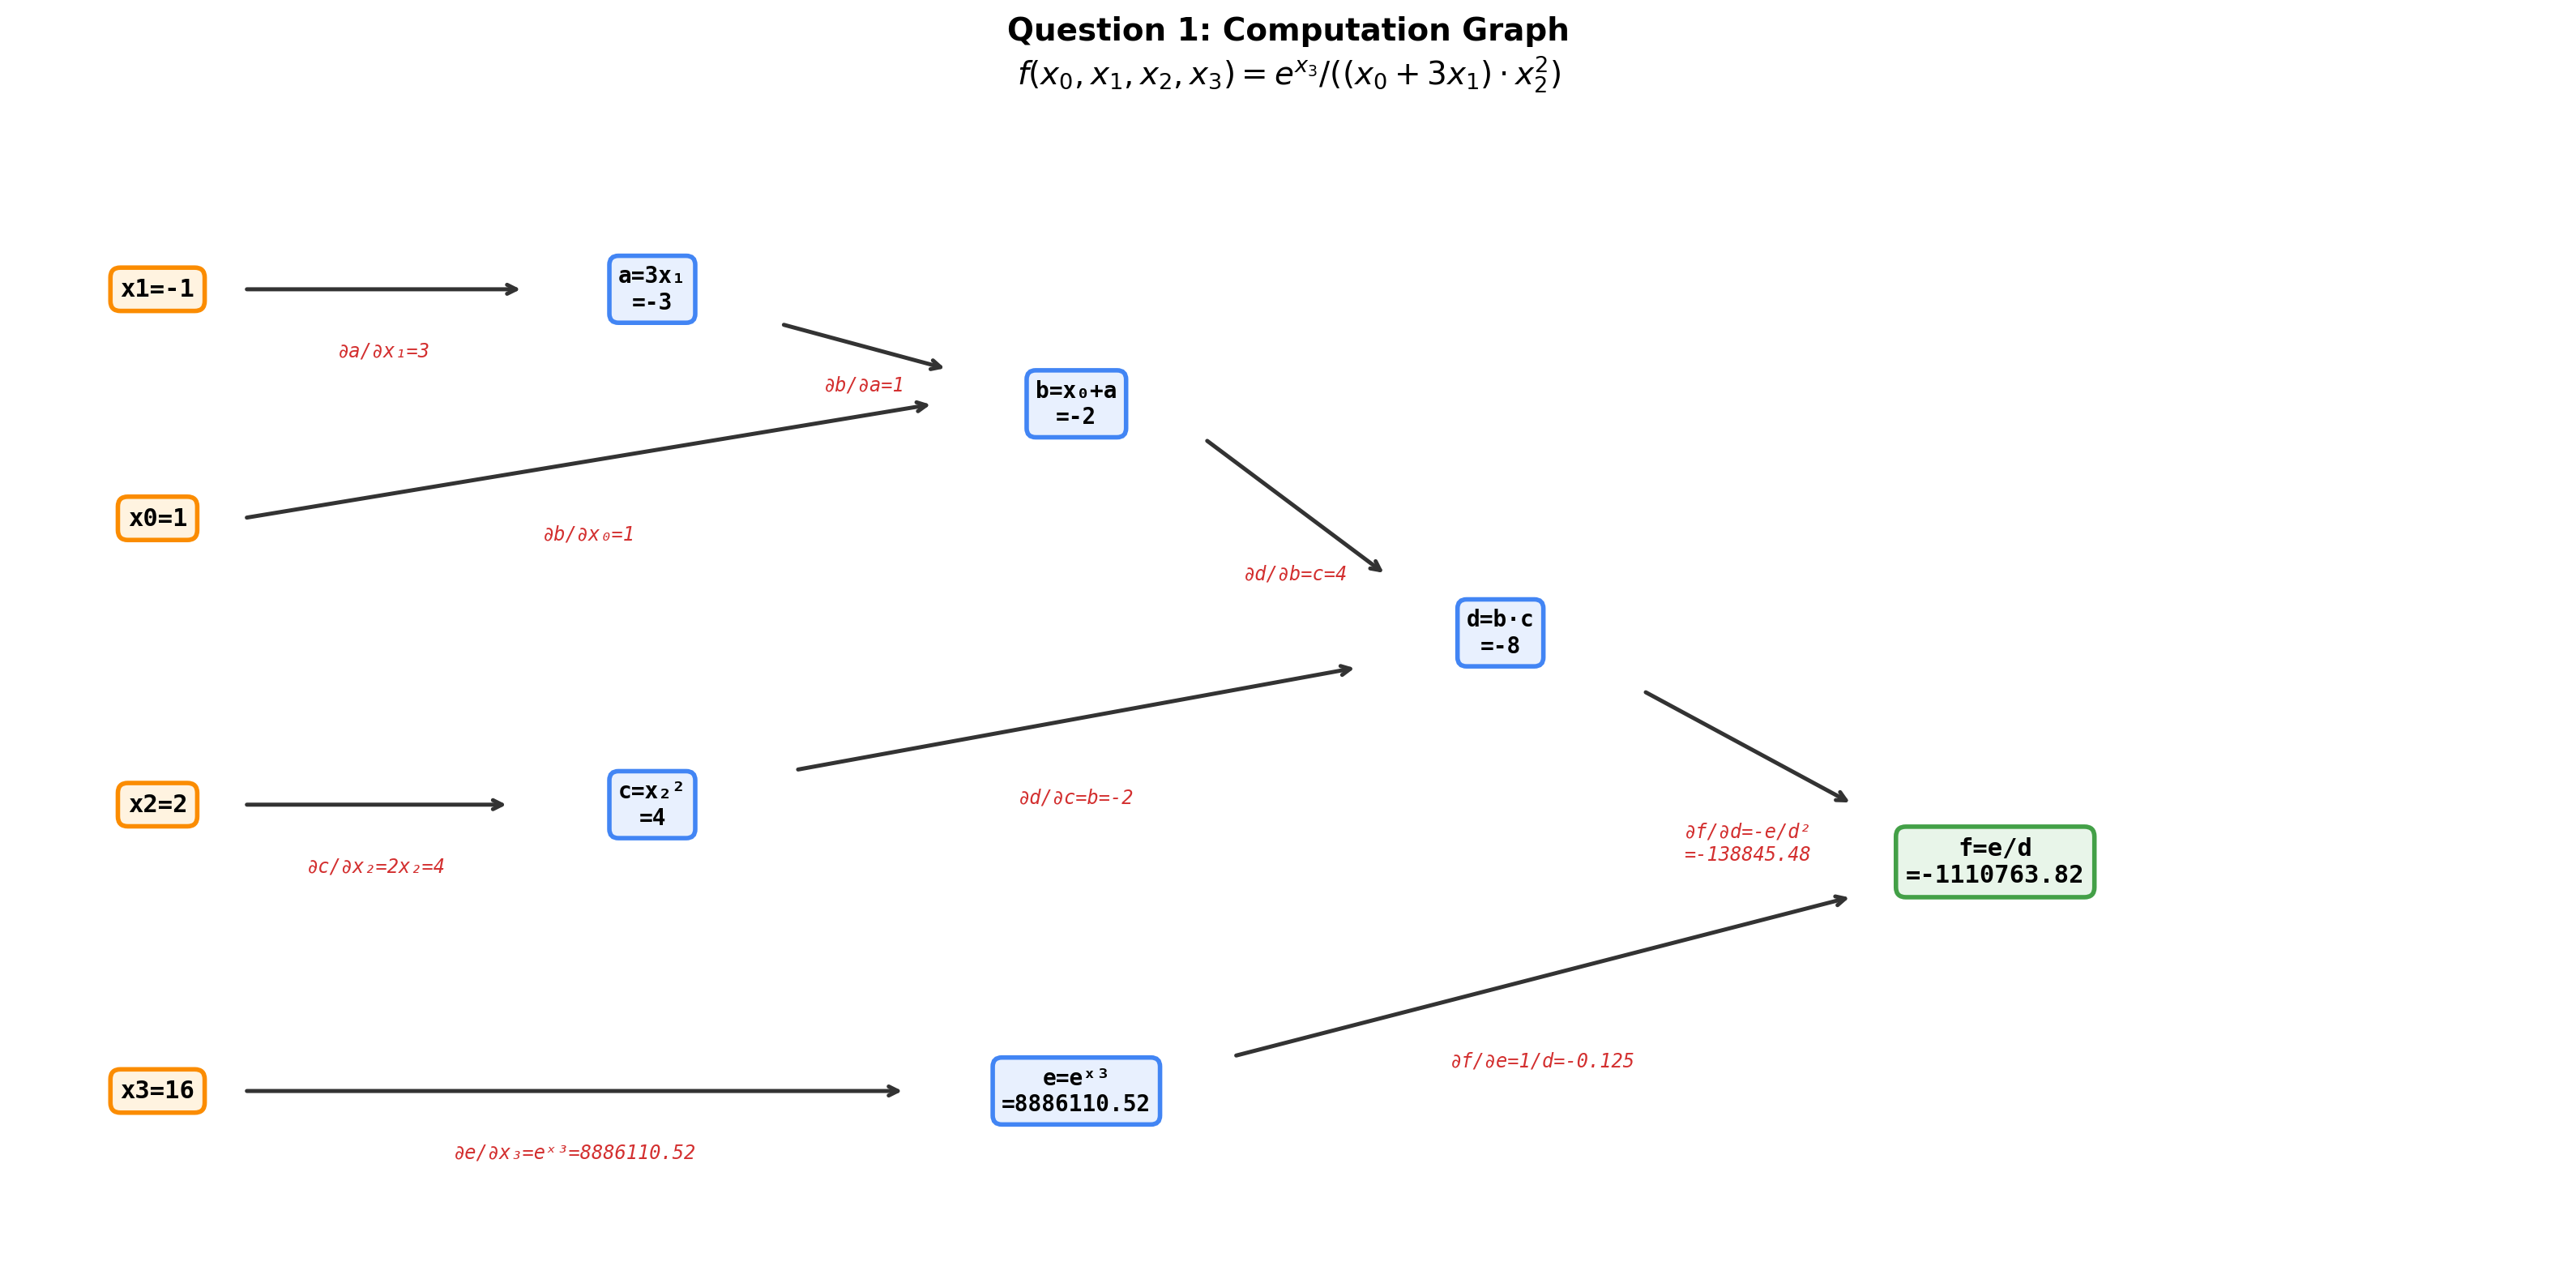
\includegraphics[width=0.95\textwidth]{q1_computation_graph.png}
\caption{Computation graph of $f(x_0, x_1, x_2, x_3)$ with forward outputs (above edges) and local gradients (below edges).}
\end{figure}

\subsection{Forward Pass --- Intermediate Outputs}

\begin{table}[H]
\centering
\caption{Intermediate outputs of the forward pass}
\begin{tabular}{ccc}
\toprule
\textbf{Node} & \textbf{Expression} & \textbf{Value} \\
\midrule
$a$ & $3 \times x_1 = 3 \times (-1)$ & $-3$ \\
$b$ & $x_0 + a = 1 + (-3)$ & $-2$ \\
$c$ & $x_2^2 = 2^2$ & $4$ \\
$d$ & $b \times c = (-2) \times 4$ & $-8$ \\
$e$ & $e^{x_3} = e^{16}$ & $8{,}886{,}110.52$ \\
$f$ & $e / d = 8{,}886{,}110.52 / (-8)$ & $-1{,}110{,}763.82$ \\
\bottomrule
\end{tabular}
\end{table}

\subsection{Backward Pass --- Gradients (Chain Rule)}

\begin{table}[H]
\centering
\caption{Gradients computed via the chain rule (backward pass)}
\begin{tabular}{ccc}
\toprule
\textbf{Gradient} & \textbf{Derivation} & \textbf{Value} \\
\midrule
$\frac{\partial f}{\partial f}$ & $1$ & $1$ \\[4pt]
$\frac{\partial f}{\partial e}$ & $\frac{1}{d} = \frac{1}{-8}$ & $-0.125$ \\[4pt]
$\frac{\partial f}{\partial d}$ & $-\frac{e}{d^2} = -\frac{8{,}886{,}110.52}{64}$ & $-138{,}845.48$ \\[4pt]
$\frac{\partial f}{\partial x_3}$ & $\frac{\partial f}{\partial e} \cdot e^{x_3} = \frac{e^{x_3}}{d}$ & $-1{,}110{,}763.82$ \\[4pt]
$\frac{\partial f}{\partial b}$ & $\frac{\partial f}{\partial d} \cdot c = (-138{,}845.48) \times 4$ & $-555{,}381.91$ \\[4pt]
$\frac{\partial f}{\partial c}$ & $\frac{\partial f}{\partial d} \cdot b = (-138{,}845.48) \times (-2)$ & $277{,}690.95$ \\[4pt]
$\frac{\partial f}{\partial x_0}$ & $\frac{\partial f}{\partial b} \cdot \frac{\partial b}{\partial x_0} = (-555{,}381.91) \times 1$ & $\mathbf{-555{,}381.91}$ \\[4pt]
$\frac{\partial f}{\partial x_1}$ & $\frac{\partial f}{\partial b} \cdot \frac{\partial b}{\partial a} \cdot \frac{\partial a}{\partial x_1} = (-555{,}381.91) \times 1 \times 3$ & $\mathbf{-1{,}666{,}145.72}$ \\[4pt]
$\frac{\partial f}{\partial x_2}$ & $\frac{\partial f}{\partial c} \cdot \frac{\partial c}{\partial x_2} = 277{,}690.95 \times 2x_2 = 277{,}690.95 \times 4$ & $\mathbf{1{,}110{,}763.82}$ \\[4pt]
\bottomrule
\end{tabular}
\end{table}

\subsection{Final Gradients Summary}
\begin{itemize}[nosep]
\item $\frac{\partial f}{\partial x_0} = -555{,}381.91$
\item $\frac{\partial f}{\partial x_1} = -1{,}666{,}145.72$
\item $\frac{\partial f}{\partial x_2} = 1{,}110{,}763.82$
\item $\frac{\partial f}{\partial x_3} = -1{,}110{,}763.82$
\end{itemize}

\noindent\textit{(Verified with PyTorch autograd --- results match.)}

\newpage

% ============================================================
\section{Question 2: 2-Cluster --- Observations (40 points)}

After training single-hidden-layer MLPs with hidden units of 2, 5, 10, 50, 100, 500, 1000, and 5000 on the 2-cluster dataset, the following observations are made.

\subsection{Test Accuracy vs.\ Number of Hidden Units}

\begin{table}[H]
\centering
\caption{Test accuracy for different numbers of hidden units}
\begin{tabular}{lcccccccc}
\toprule
\textbf{Hidden Units} & 2 & 5 & 10 & 50 & 100 & 500 & 1000 & 5000 \\
\midrule
\textbf{Accuracy} & 36.5\% & 44.5\% & 62.0\% & 86.5\% & 88.0\% & 88.0\% & 89.0\% & 90.5\% \\
\bottomrule
\end{tabular}
\end{table}

\begin{figure}[H]
\centering
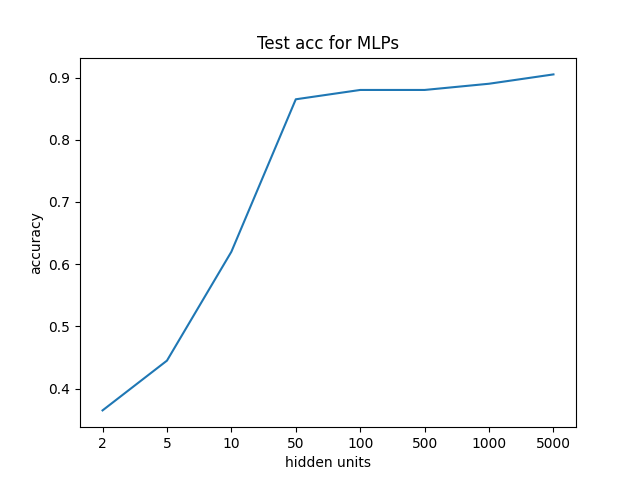
\includegraphics[width=0.65\textwidth]{2_cluster_test_acc.png}
\caption{Test accuracy as a function of the number of hidden units.}
\end{figure}

\subsection{Observations}

\begin{enumerate}
\item \textbf{Accuracy increases with hidden units.}
As the number of hidden units increases from 2 to 5000, test accuracy improves significantly---from 36.5\% to 90.5\%. This demonstrates that higher model capacity enables the MLP to learn more complex decision boundaries.

\item \textbf{Rapid improvement in the low range.}
The most dramatic accuracy gains occur between 2 and 50 hidden units (36.5\% $\to$ 86.5\%), a nearly 50 percentage point improvement. This indicates that the 2-cluster classification task requires a moderate level of model capacity to separate the two classes.

\item \textbf{Diminishing returns at higher capacity.}
Beyond 100 hidden units, accuracy improvements become marginal (88.0\% $\to$ 90.5\%). The accuracy curve plateaus, suggesting that additional hidden units provide diminishing returns once the model has sufficient capacity to capture the decision boundary.

\item \textbf{Decision boundary complexity.}
With very few hidden units (2 or 5), the decision boundaries are nearly linear and cannot separate the two clusters effectively. As hidden units increase (50+), the boundaries become increasingly non-linear and curved, closely conforming to the shape of the data clusters. With 1000 or 5000 units, the boundaries are highly detailed and smooth.

\item \textbf{No clear overfitting observed.}
Even with 5000 hidden units (far exceeding the data complexity), the test accuracy continues to improve slightly rather than decrease, indicating that the model generalizes well within 30 training epochs. However, with more epochs, overfitting could potentially occur for very large models.
\end{enumerate}

\subsection{Decision Boundary Visualizations}

\begin{figure}[H]
\centering
\begin{minipage}{0.48\textwidth}
\centering
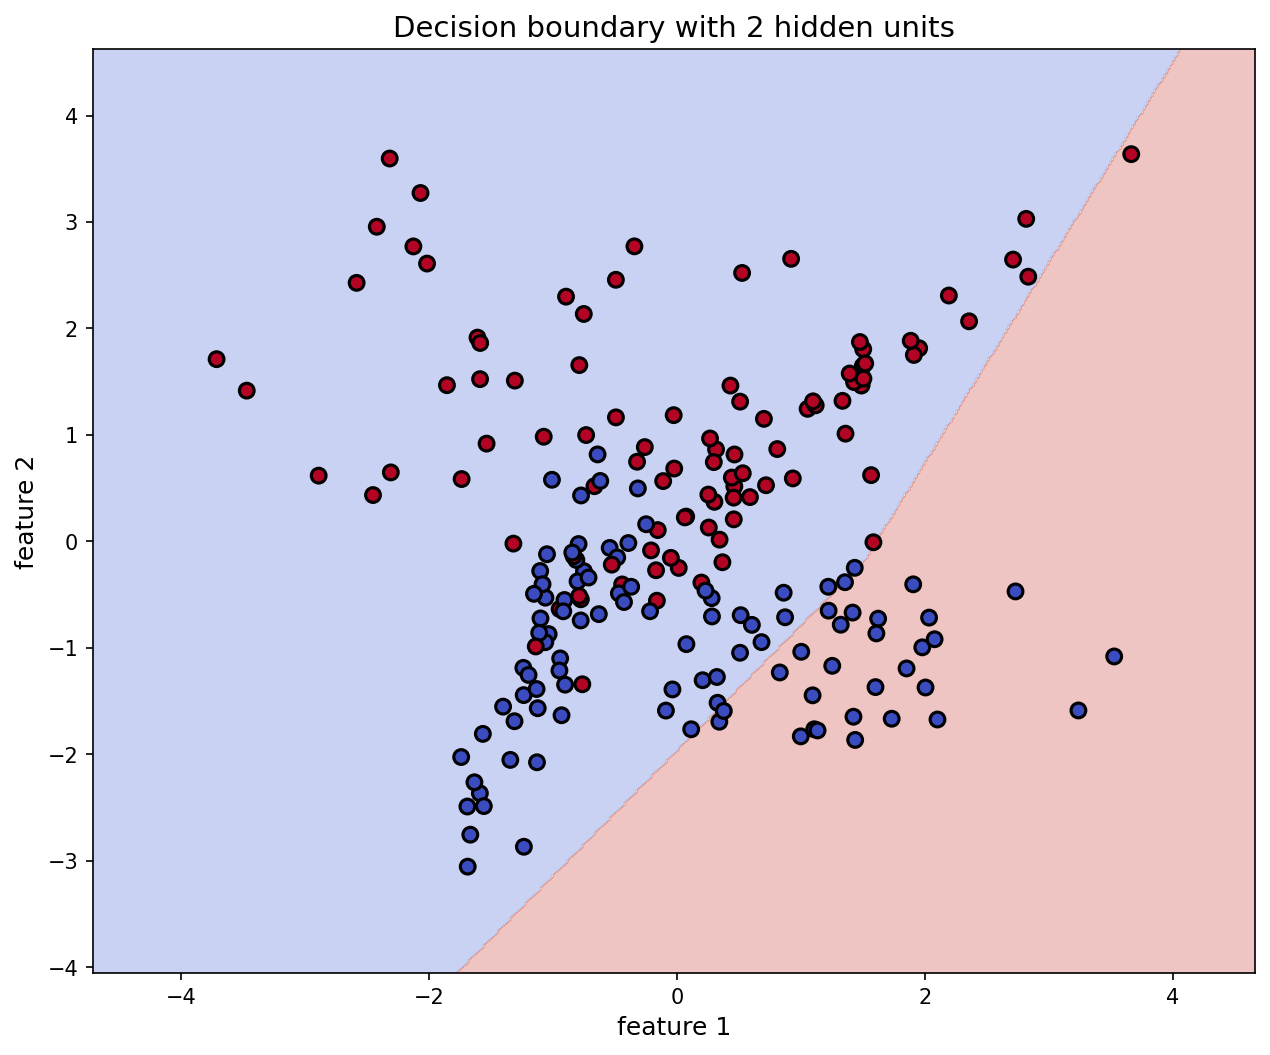
\includegraphics[width=\textwidth]{decision_boundary_2.png}
\caption{2 hidden units}
\end{minipage}\hfill
\begin{minipage}{0.48\textwidth}
\centering
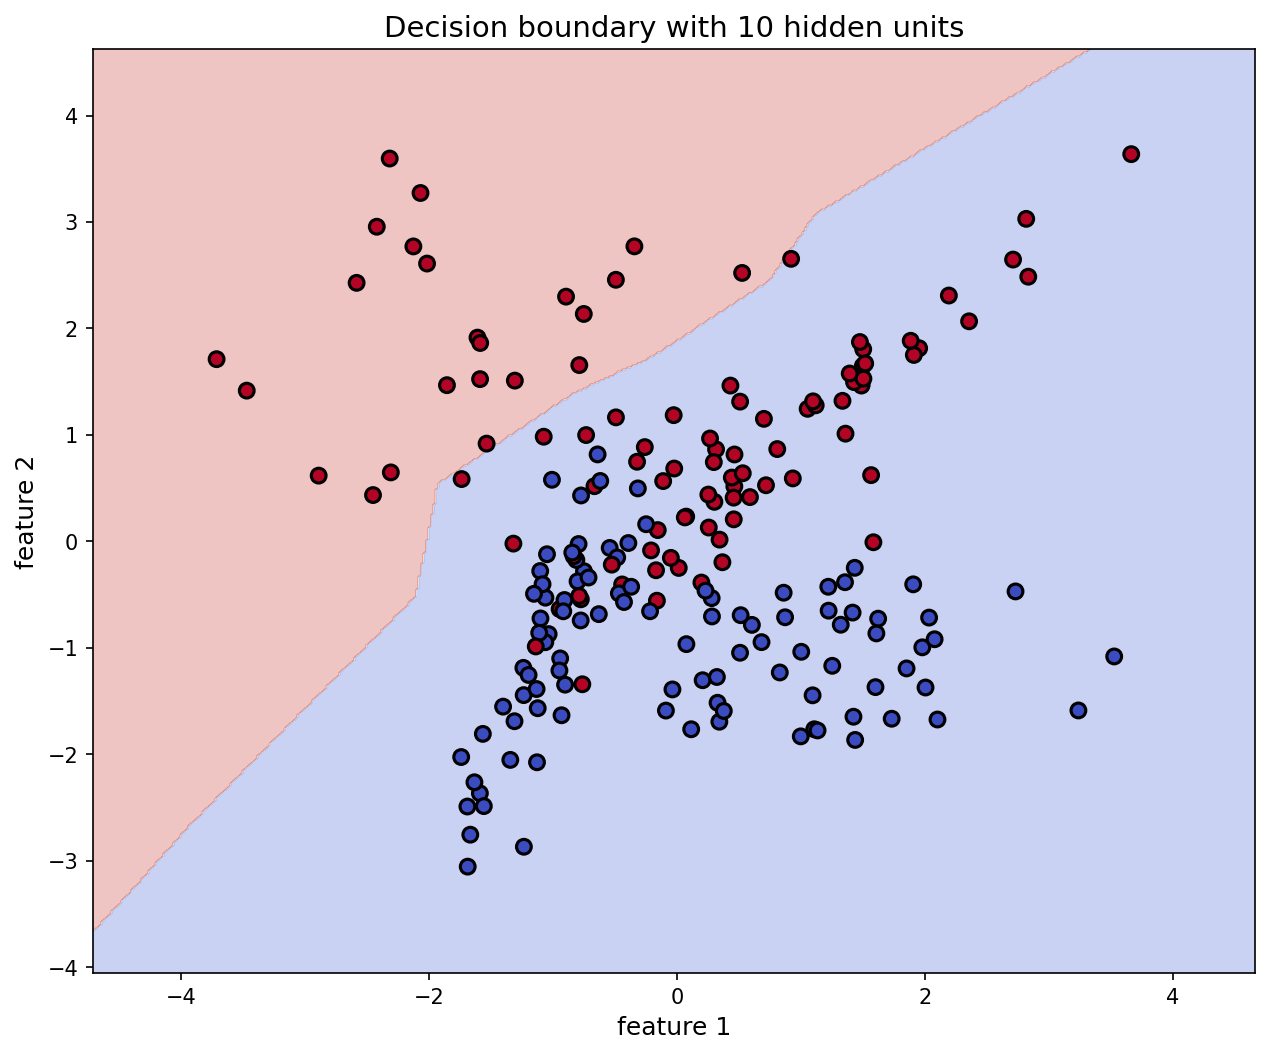
\includegraphics[width=\textwidth]{decision_boundary_10.png}
\caption{10 hidden units}
\end{minipage}
\end{figure}

\begin{figure}[H]
\centering
\begin{minipage}{0.48\textwidth}
\centering
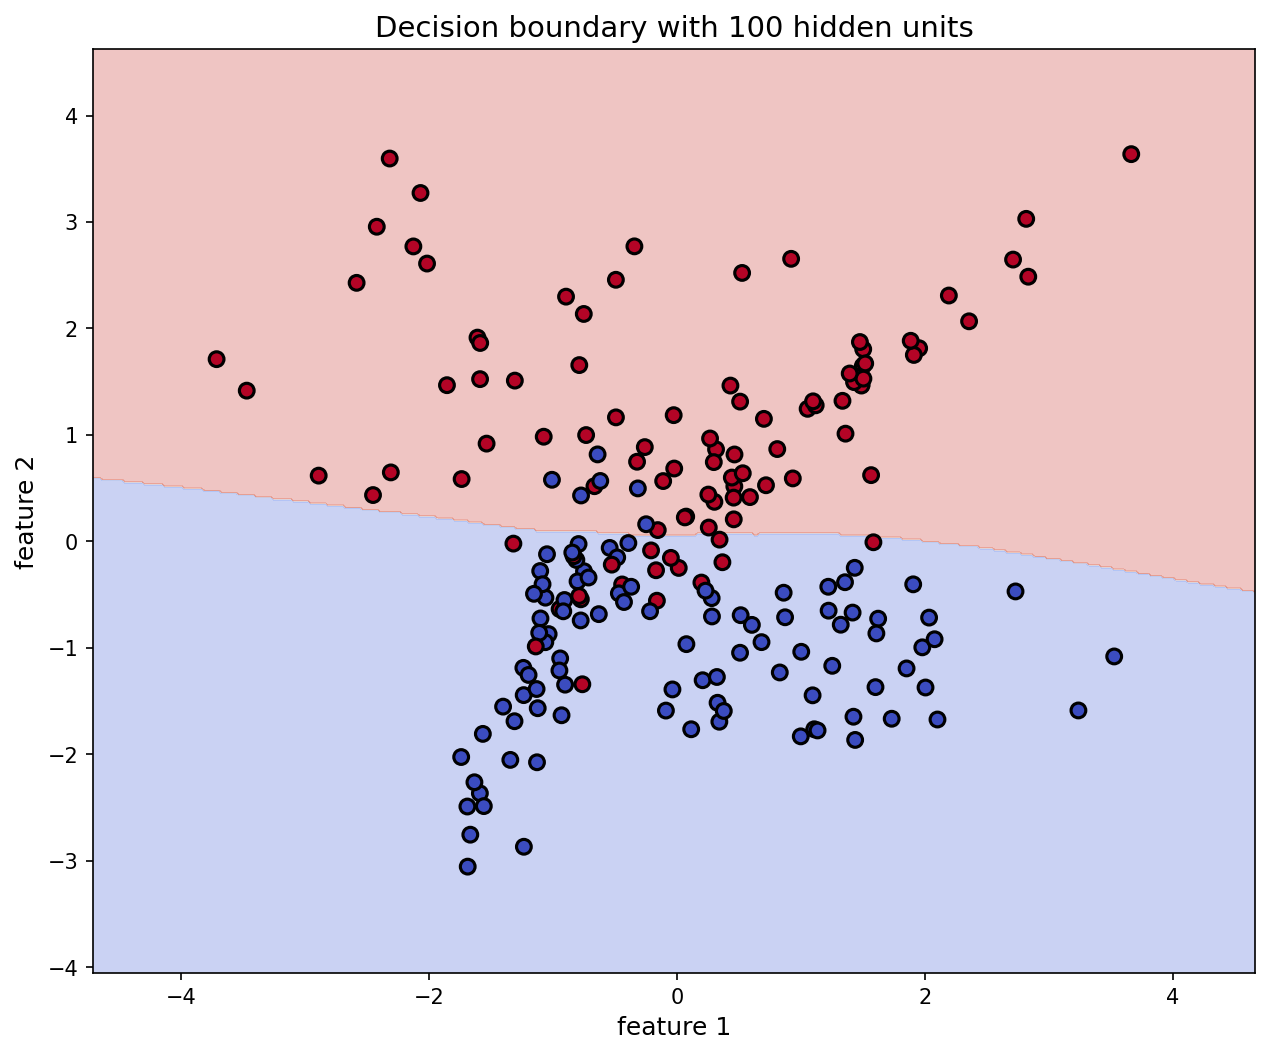
\includegraphics[width=\textwidth]{decision_boundary_100.png}
\caption{100 hidden units}
\end{minipage}\hfill
\begin{minipage}{0.48\textwidth}
\centering
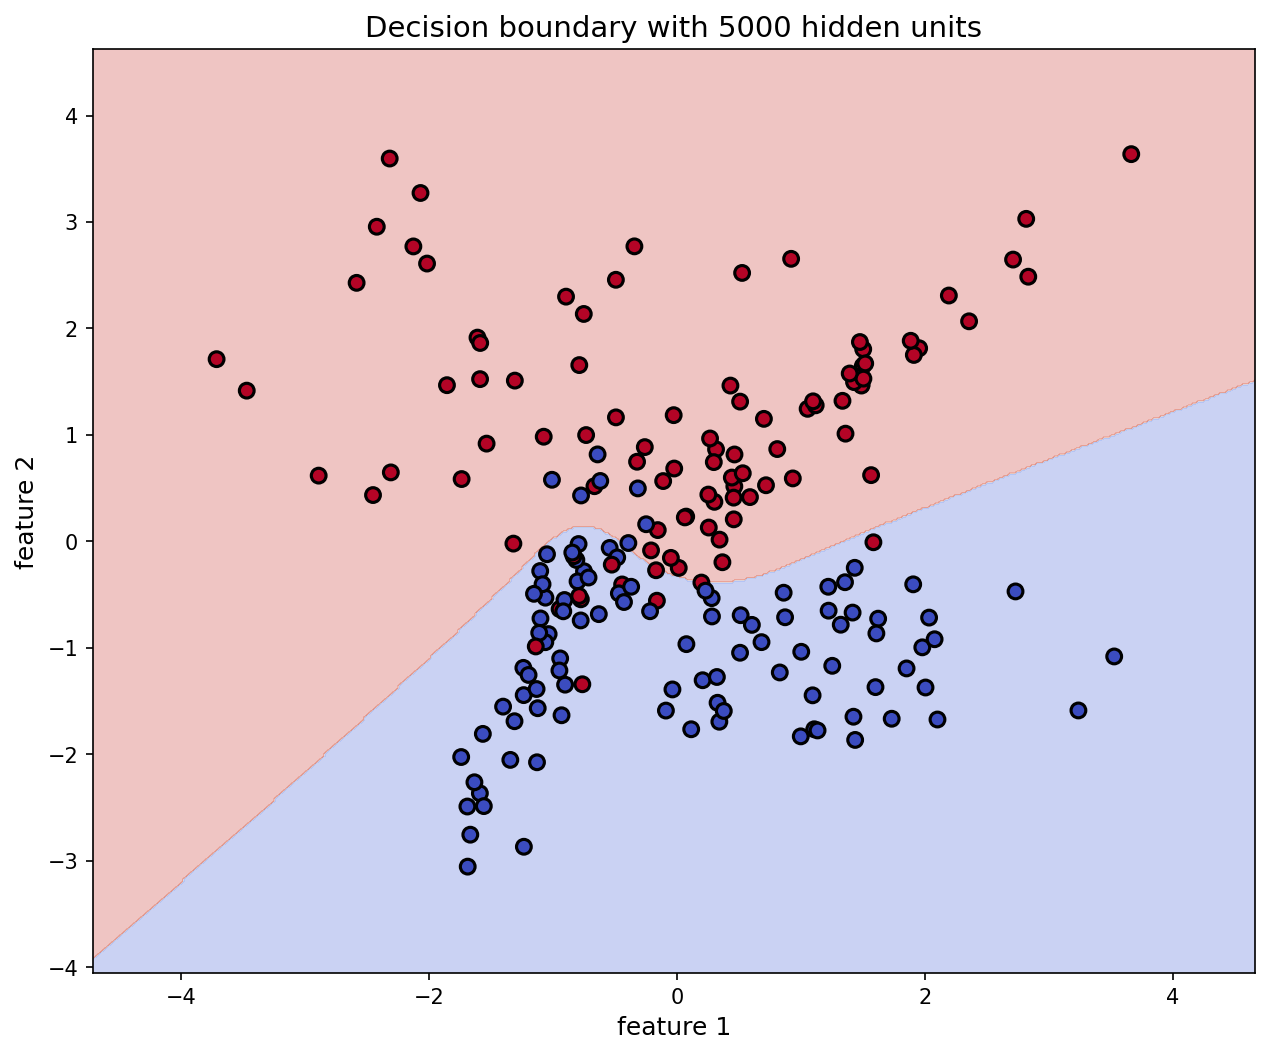
\includegraphics[width=\textwidth]{decision_boundary_5000.png}
\caption{5000 hidden units}
\end{minipage}
\end{figure}

\end{document}
